\chapter{The Lighting System}
    In this chapter, a formal definition and introduction of all system parts with an explanation of their purpose is provided. The names for system devices used in the following chapters are \textbf{Light Control Unit} and \textbf{Floating Button}, and they were taken from SCILIF directly.
    Additionally, user and functional requirements and user interactions with the system are specified.
    
    \section{Light Control Unit}
        \label{sec:urs_lcu}
        The light control unit is a battery device connected directly to the optic fibres that are encased in textile clothing. The brightness emitted by optic fibres is set by controlling the electrical current flowing through optical LED powering a light guide. There are several pre-defined levels of brightness and blinking modes called light modes (see section \ref{sec:light_modes}).
        The unit is usually placed in a pocket typically located at the back waist part of a vest or a jacket.
        
        \begin{figure}[!ht]
            \centering
    	    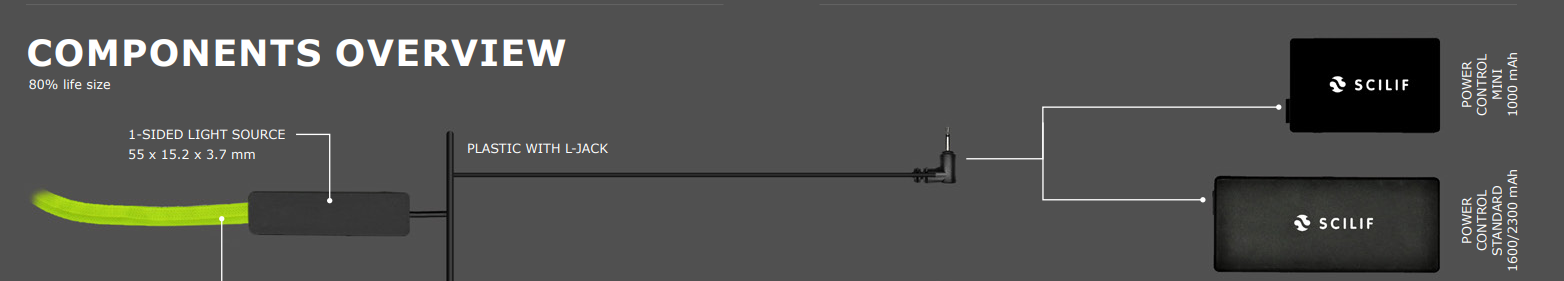
\includegraphics[width =1.1\textwidth]{URS/Figs/scilif_system01.png}
            \caption {A visualization of the light control unit}
            \label{figure:scilif_lcu}
        \end{figure}  
        
        
    \section{Floating Button}
        \label{sec:urs_fb}
         The floating button is a battery device placed on a comfortably reachable part of a vest/jacket. It allows the user remotely and quickly change the light modes on the light control unit without the need to open the smartphone/smartwatch application. Because the floating button communicates with the light control unit remotely, no connection cables are needed. Furthermore, the floating button is designed to have good haptic properties. 
       
        \begin{figure}[!ht]
            \centering
    	    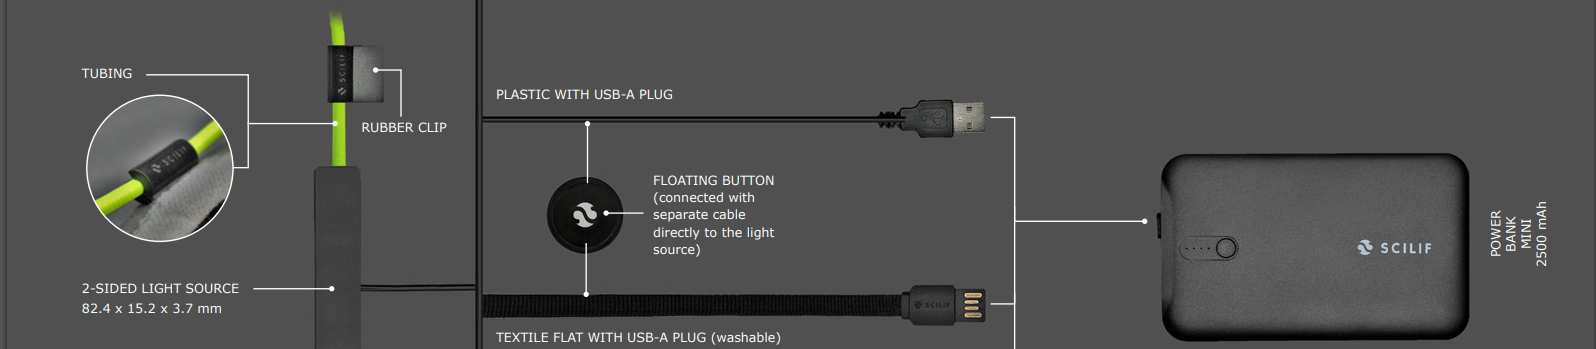
\includegraphics[width =1.1\textwidth]{URS/Figs/scilif_system02.png}
            \caption {A visualization of the floating button}
            \label{figure:scilif_fb}
        \end{figure}  
       
    \section{RFID Switch}
        The RFID switch consists of two parts - RFID reader and RFID tag. Both of them can be sewed into the clothing - the coil of RFID reader into arbitrary comfortably reachable part and the RFID tag into a sleeve. When the user wants to change the light mode, he only needs to bring the sleeve near the coil to trigger the light mode change. Due to the fact that the RFID reader has to be physically connected to the light control unit, wires must be stitched onto the clothing. 
       
       
    \section{Light Modes}  
    \label{sec:light_modes}
        As the most important user interaction with the system, the light control unit allows turning on/off the lighting or changing the predefined light modes. At the time of writing, five different light modes were defined:
        
        \begin{enumerate}
            \item No Lighting 
            \item Strong Lighting (145 mA)
            \item Low Lighting (60 mA)
            \item Slow Blinking (2 s period)
            \item Fast Blinking (0.5 s period).
        \end{enumerate}
        
        Both blinking modes use strong lighting (145 mA), and the duty cycle is 50 \%. These numbers were defined according to SCILIF requirements.
        
        The state of the art of this problem is to develop a satisfying way how to change these light modes. The considerations were given on how practical and comfortable the solution is, as well as on meeting the client's functional requirements, such as maintaining low power consumption, reducing the additional costs, etc. 
       
       \subsection{Methods for changing the light modes}
        \label{sec:light_modes_methods}
        
        During the work on the thesis, multiple ways how to change the light modes were implemented. The direct change to preferred light mode is possible only through mobile/smartwatch application. All other methods simply increment the current mode.
        The list below shows all of them.
        
        \begin{itemize}
            \item Pressing button on the light control unit
            \item Remote change over BLE by mobile/smartwatch application
            \item Remote change over BLE by tapping on the floating button
            \item RFID switch
            \item Gesture control (not implemented yet) 
        \end{itemize}
        

        Since the spectrum of end-users is large, particular methods might suit different customer needs or use cases. The most relevant questions that should be addressed are: \\
        
        \begin{itemize}
        \setlength\itemsep{0em}
            \item  How to change the light mode when the unit is not reachable by hands. The unit might be encased in the clothing, or it might be located in the back pocket. \\
            \item How to change the light modes quickly, with the least possible effort (for example, in the case of a motorbike driver or a biker). 
        \end{itemize}
        
        
        A quick analysis of these methods:
        
        \textbf{Change by pressing the button on the light control unit directly} brings no overhead in terms of costs and battery usage. Nevertheless, it is the less practical method, and in many use cases, it is not applicable at all.
        
        \textbf{Remote change by mobile/smartwatch application} is based on BLE communication between the central (mobile phone/smartwatch) and peripheral (light control unit). Initially, the light control unit needs to be bonded and connected to the central.\\
        The advantage of this method is that it allows changing the light modes even though the unit is not reachable. On the other hand, one still needs to take a mobile phone and open the mobile application, so it is not very practical in the use cases when a quick change is desired. This method also increases the overall cost and battery consumption since a BLE-based MCU must be used.
        
        \textbf{Change by RFID switch} is based on the inductive coupling principle. When the user brings the sleeve with encased RFID tag close to the reader, it triggers the change of a light mode.\\
	    This method addresses both questions defined above. On the contrary, the biggest drawback of this method is the increased battery consumption needed for checking the incoming RFID transmissions. Besides that, the cables between the coil of RFID reader and the unit must be sewed into the clothing and the probability of unwanted switches increases.
        
        \textbf{Remote change by tapping on the floating button} is based on BLE communication between the central (floating button) and the peripheral (light control unit). The light control unit needs to be bonded and connected to the central.\\
        Apart from solving both constraints defined above, this method also does not require any wiring. Nevertheless, it brings the biggest overhead in terms of the costs since two BLE devices must be used.
        
        \textbf{Change by a gesture} allows the user to change the light mode by a predefined gesture. It is rather an experimental feature.
        
        
        Last but not least, one should take into account that these methods could be combined, and it always depends on the use case and customer's preferences.
        
    \section{Maintenance}
       Considering the fact that both the light control unit and floating button are battery devices, the system should be able to provide information such as battery level,  charging status or temperature. These so-called maintenance data can be obtained via BLE using a mobile/smartwatch application.

        Another user's interaction with the system is the OTA (Over The Air) firmware upgrade that enables users to flash a new firmware version through a mobile application over BLE.

        Both of these are possible only with BLE-based MCU.
        
        
        
        